% Generated by LitigCharts.PublicationFigures. Captions and provenance are sidecars.
\documentclass[10pt,tikz,border=5pt]{standalone}
\usepackage{lmodern}
\usetikzlibrary{patterns,patterns.meta}
\begin{document}
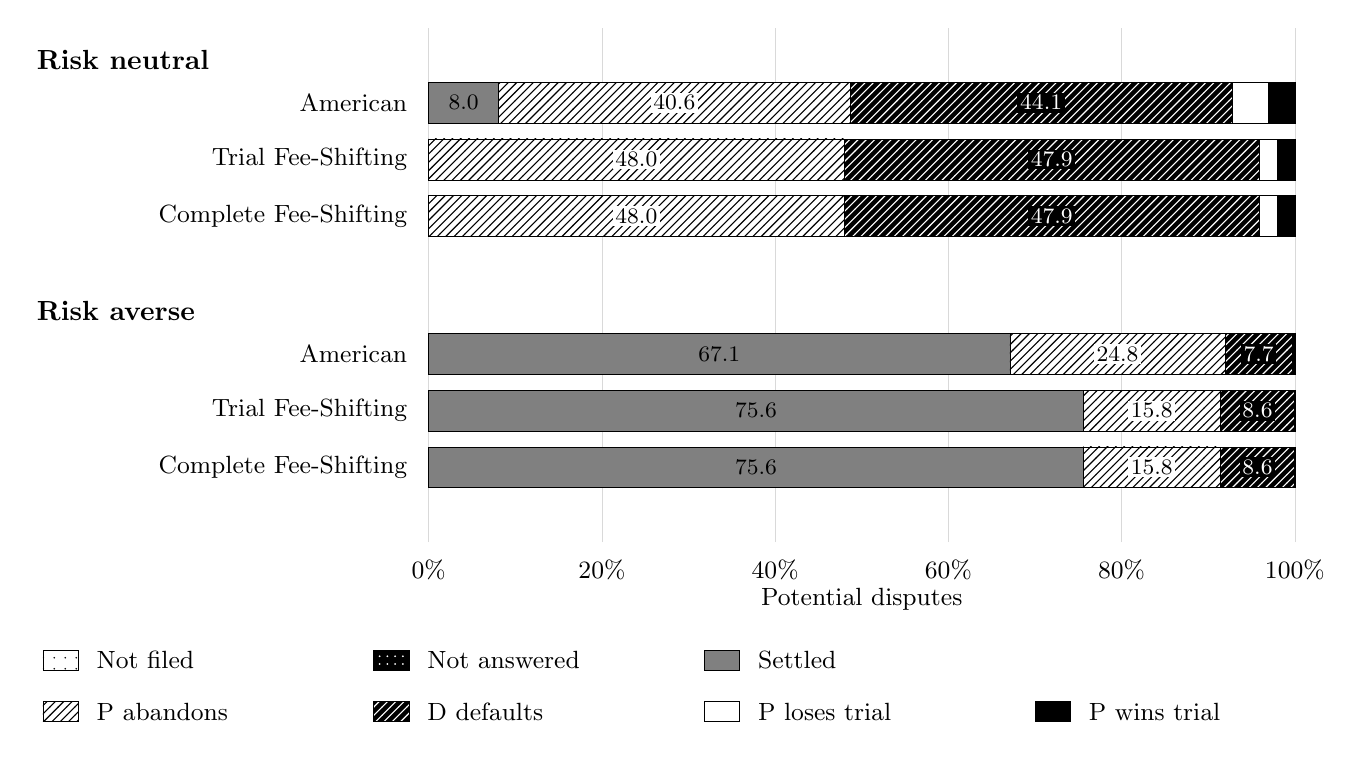
\begin{tikzpicture}[font=\small]\draw[black!15,line width=.2pt] (5.1,.65) -- (5.1,7.18);
\node[anchor=north] at (5.1,.55) {0\%};
\draw[black!15,line width=.2pt] (7.3,.65) -- (7.3,7.18);
\node[anchor=north] at (7.3,.55) {20\%};
\draw[black!15,line width=.2pt] (9.5,.65) -- (9.5,7.18);
\node[anchor=north] at (9.5,.55) {40\%};
\draw[black!15,line width=.2pt] (11.7,.65) -- (11.7,7.18);
\node[anchor=north] at (11.7,.55) {60\%};
\draw[black!15,line width=.2pt] (13.9,.65) -- (13.9,7.18);
\node[anchor=north] at (13.9,.55) {80\%};
\draw[black!15,line width=.2pt] (16.1,.65) -- (16.1,7.18);
\node[anchor=north] at (16.1,.55) {100\%};
\node[anchor=west,font=\bfseries] at (0,6.78) {\mbox{Risk} \mbox{neutral}};
\node[anchor=east] at (4.95,6.23) {American};
\path[fill=black!50,draw=black,line width=.25pt] (5.1,5.97) rectangle (5.984924,6.49);
\node[text=black,fill=none,font=\footnotesize,inner sep=1pt] at (5.542462,6.23) {8.0};
\path[preaction={fill=white,draw=none},pattern={north east lines},pattern color=black,draw=black,line width=.25pt] (5.984924,5.97) rectangle (10.455175,6.49);
\node[text=black,fill=white,font=\footnotesize,inner sep=1pt] at (8.220049,6.23) {40.6};
\path[preaction={fill=black,draw=none},pattern={north east lines},pattern color=white,draw=black,line width=.25pt] (10.455175,5.97) rectangle (15.300824,6.49);
\node[text=white,fill=black,font=\footnotesize,inner sep=1pt] at (12.877999,6.23) {44.1};
\path[fill=white,draw=black,line width=.25pt] (15.300824,5.97) rectangle (15.760983,6.49);
\path[fill=black,draw=black,line width=.25pt] (15.760983,5.97) rectangle (16.100003,6.49);
\node[anchor=east] at (4.95,5.51) {Trial Fee-Shifting};
\path[preaction={fill=white,draw=none},pattern={north east lines},pattern color=black,draw=black,line width=.25pt] (5.1,5.25) rectangle (10.374555,5.77);
\node[text=black,fill=white,font=\footnotesize,inner sep=1pt] at (7.737278,5.51) {48.0};
\path[preaction={fill=black,draw=none},pattern={north east lines},pattern color=white,draw=black,line width=.25pt] (10.374555,5.25) rectangle (15.648945,5.77);
\node[text=white,fill=black,font=\footnotesize,inner sep=1pt] at (13.01175,5.51) {47.9};
\path[fill=white,draw=black,line width=.25pt] (15.648945,5.25) rectangle (15.87448,5.77);
\path[fill=black,draw=black,line width=.25pt] (15.87448,5.25) rectangle (16.100004,5.77);
\node[anchor=east] at (4.95,4.79) {Complete Fee-Shifting};
\path[preaction={fill=white,draw=none},pattern={north east lines},pattern color=black,draw=black,line width=.25pt] (5.1,4.53) rectangle (10.374555,5.05);
\node[text=black,fill=white,font=\footnotesize,inner sep=1pt] at (7.737278,4.79) {48.0};
\path[preaction={fill=black,draw=none},pattern={north east lines},pattern color=white,draw=black,line width=.25pt] (10.374555,4.53) rectangle (15.648945,5.05);
\node[text=white,fill=black,font=\footnotesize,inner sep=1pt] at (13.01175,4.79) {47.9};
\path[fill=white,draw=black,line width=.25pt] (15.648945,4.53) rectangle (15.87448,5.05);
\path[fill=black,draw=black,line width=.25pt] (15.87448,4.53) rectangle (16.100004,5.05);
\node[anchor=west,font=\bfseries] at (0,3.59) {\mbox{Risk} \mbox{averse}};
\node[anchor=east] at (4.95,3.04) {American};
\path[fill=black!50,draw=black,line width=.25pt] (5.1,2.78) rectangle (12.4821,3.3);
\node[text=black,fill=none,font=\footnotesize,inner sep=1pt] at (8.79105,3.04) {67.1};
\path[preaction={fill=white,draw=none},pattern={north east lines},pattern color=black,draw=black,line width=.25pt] (12.4821,2.78) rectangle (15.21527,3.3);
\node[text=black,fill=white,font=\footnotesize,inner sep=1pt] at (13.848685,3.04) {24.8};
\path[preaction={fill=black,draw=none},pattern={north east lines},pattern color=white,draw=black,line width=.25pt] (15.21527,2.78) rectangle (16.066132,3.3);
\node[text=white,fill=black,font=\footnotesize,inner sep=1pt] at (15.640701,3.04) {7.7};
\path[fill=white,draw=black,line width=.25pt] (16.066132,2.78) rectangle (16.076108,3.3);
\path[fill=black,draw=black,line width=.25pt] (16.076108,2.78) rectangle (16.1,3.3);
\node[anchor=east] at (4.95,2.32) {Trial Fee-Shifting};
\path[fill=black!50,draw=black,line width=.25pt] (5.1,2.06) rectangle (13.411534,2.58);
\node[text=black,fill=none,font=\footnotesize,inner sep=1pt] at (9.255767,2.32) {75.6};
\path[preaction={fill=white,draw=none},pattern={north east lines},pattern color=black,draw=black,line width=.25pt] (13.411534,2.06) rectangle (15.154645,2.58);
\node[text=black,fill=white,font=\footnotesize,inner sep=1pt] at (14.28309,2.32) {15.8};
\path[preaction={fill=black,draw=none},pattern={north east lines},pattern color=white,draw=black,line width=.25pt] (15.154645,2.06) rectangle (16.096805,2.58);
\node[text=white,fill=black,font=\footnotesize,inner sep=1pt] at (15.625725,2.32) {8.6};
\path[fill=white,draw=black,line width=.25pt] (16.096805,2.06) rectangle (16.098214,2.58);
\path[fill=black,draw=black,line width=.25pt] (16.098214,2.06) rectangle (16.1,2.58);
\node[anchor=east] at (4.95,1.6) {Complete Fee-Shifting};
\path[fill=black!50,draw=black,line width=.25pt] (5.1,1.34) rectangle (13.411534,1.86);
\node[text=black,fill=none,font=\footnotesize,inner sep=1pt] at (9.255767,1.6) {75.6};
\path[preaction={fill=white,draw=none},pattern={north east lines},pattern color=black,draw=black,line width=.25pt] (13.411534,1.34) rectangle (15.154645,1.86);
\node[text=black,fill=white,font=\footnotesize,inner sep=1pt] at (14.28309,1.6) {15.8};
\path[preaction={fill=black,draw=none},pattern={north east lines},pattern color=white,draw=black,line width=.25pt] (15.154645,1.34) rectangle (16.096805,1.86);
\node[text=white,fill=black,font=\footnotesize,inner sep=1pt] at (15.625725,1.6) {8.6};
\path[fill=white,draw=black,line width=.25pt] (16.096805,1.34) rectangle (16.098214,1.86);
\path[fill=black,draw=black,line width=.25pt] (16.098214,1.34) rectangle (16.1,1.86);
\node at (10.6,-.08) {Potential disputes};
\path[preaction={fill=white,draw=none},pattern={Dots[distance=4pt,radius=.35pt]},pattern color=black,draw=black,line width=.25pt] (0.2,-0.98) rectangle (0.65,-0.72);
\node[anchor=west] at (0.76,-0.85) {Not filed};
\path[preaction={fill=black,draw=none},pattern={Dots[distance=2.8pt,radius=.35pt]},pattern color=white,draw=black,line width=.25pt] (4.4,-0.98) rectangle (4.85,-0.72);
\node[anchor=west] at (4.96,-0.85) {Not answered};
\path[fill=black!50,draw=black,line width=.25pt] (8.6,-0.98) rectangle (9.05,-0.72);
\node[anchor=west] at (9.16,-0.85) {Settled};
\path[preaction={fill=white,draw=none},pattern={north east lines},pattern color=black,draw=black,line width=.25pt] (0.2,-1.63) rectangle (0.65,-1.37);
\node[anchor=west] at (0.76,-1.5) {P abandons};
\path[preaction={fill=black,draw=none},pattern={north east lines},pattern color=white,draw=black,line width=.25pt] (4.4,-1.63) rectangle (4.85,-1.37);
\node[anchor=west] at (4.96,-1.5) {D defaults};
\path[fill=white,draw=black,line width=.25pt] (8.6,-1.63) rectangle (9.05,-1.37);
\node[anchor=west] at (9.16,-1.5) {P loses trial};
\path[fill=black,draw=black,line width=.25pt] (12.8,-1.63) rectangle (13.25,-1.37);
\node[anchor=west] at (13.36,-1.5) {P wins trial};
\end{tikzpicture}
\end{document}
